\chapter{Forced Oscillations and Resonance}

The previous chapter closed with a brief preview of the damped oscillator. We now develop it in full, and then take the decisive step of driving the oscillator with an external periodic force. Two phenomena emerge that have no counterpart in the free oscillator: the transient decay of any initial disturbance, and the dramatic amplification of the steady response when the drive is tuned near the natural frequency --- resonance. Both are governed by a single new parameter, the damping rate $\Gamma$, and much of the chapter is an exploration of how that one number controls the timescale of decay, the sharpness of the resonance, and the phase relationship between drive and response.

% ============================================================
\section{Damped Oscillators}
% ============================================================

Suppose the mass--spring system is immersed in a viscous medium, as in Figure~\ref{fig:driven-schematic}. To an ideal spring we now add a dashpot --- a piston moving in a fluid --- that exerts a frictional force proportional to the velocity and opposed to the motion,
\begin{equation}
    f = -m\Gamma\,\dot{x}, \qquad [\Gamma] = T^{-1},
\end{equation}
so Newton's second law becomes the linear, homogeneous, time-translation-invariant equation of motion
\begin{formula}
\begin{equation}
    \ddot{x}(t) + \Gamma\,\dot{x}(t) + \omega_0^2\,x(t) = 0, \qquad \omega_0 = \sqrt{k/m}.
\end{equation}
\end{formula}

\begin{figure}[ht]
\centering
\begin{tikzpicture}[>=Stealth, line width=0.8pt]
    % wall
    \fill[pattern=north east lines] (-0.35,-1.5) rectangle (0,1.5);
    \draw[line width=1pt] (0,-1.5) -- (0,1.5);
    % spring (top branch)
    \draw[decoration={coil, aspect=0.6, segment length=4.5pt, amplitude=5pt}, decorate]
        (0,0.8) -- (3,0.8);
    \node at (1.5,1.35) {$k$};
    % dashpot (bottom branch)
    \draw (0,-0.8) -- (1.0,-0.8);
    \draw (1.55,-0.5) -- (1.0,-0.5) -- (1.0,-1.1) -- (1.55,-1.1); % casing, open right
    \draw[line width=1.1pt] (1.45,-1.05) -- (1.45,-0.55);         % piston plate
    \draw (1.45,-0.8) -- (3,-0.8);                                % piston rod
    \node at (1.1,-1.45) {$m\Gamma$};
    % mass
    \draw[fill=LightGray] (3,-1.15) rectangle (4.3,1.15);
    \node at (3.65,0) {$m$};
    % driving force
    \draw[->, line width=1pt] (4.3,0) -- (5.6,0) node[right] {$F(t)$};
    % displacement coordinate
    \draw[->] (3.15,1.55) -- (4.15,1.55) node[midway, above] {$x$};
    \draw[dashed] (3.65,1.15) -- (3.65,1.7);
\end{tikzpicture}
\caption{The driven damped oscillator. An ideal spring (constant $k$) and a viscous dashpot (damping coefficient $m\Gamma$) act in parallel on the mass $m$, which is also subject to an external drive $F(t)$. Setting $F(t)=0$ recovers the free damped oscillator studied first; the general driven case is treated in Section~\ref{sec:forced}.}
\label{fig:driven-schematic}
\end{figure}

Because the equation has constant coefficients (time-translation invariant) and is linear, we seek complex solutions of the form $z(t) = e^{\alpha t}$ with $\alpha \in \mathbb{C}$. Plugging in and dividing through by $e^{\alpha t}$ gives the characteristic equation
\begin{equation}
    \alpha^2 + \Gamma\alpha + \omega_0^2 = 0
    \quad\Longrightarrow\quad
    \alpha = -\frac{\Gamma}{2} \pm \sqrt{\frac{\Gamma^2}{4} - \omega_0^2}.
\end{equation}

\begin{fact}[Damped characteristic roots]
The two roots of the damped oscillator equation are
\begin{equation}
    \alpha_\pm = -\frac{\Gamma}{2} \pm \sqrt{\frac{\Gamma^2}{4} - \omega_0^2}.
\end{equation}
The sign of the discriminant $\Gamma^2/4 - \omega_0^2$ determines the qualitative behaviour.
\end{fact}

The physics of the discriminant is intuitive. When friction dominates the natural restoring force ($\Gamma/2 > \omega_0$), the mass is unable to overshoot equilibrium and the motion is purely dissipative. When the restoring force dominates ($\Gamma/2 < \omega_0$), the mass overshoots and rings while its amplitude bleeds away. The borderline case ($\Gamma/2 = \omega_0$) is a mathematical degeneracy that also happens to be practically optimal, as we will see. We take these three regimes in turn.

\subsection{Overdamped: $\Gamma/2 > \omega_0$}

The discriminant is positive, so the square root is real and satisfies
\begin{equation}
    \sqrt{\frac{\Gamma^2}{4} - \omega_0^2} < \frac{\Gamma}{2}.
\end{equation}
Consequently both roots $\alpha_\pm$ are real and \emph{negative}. The general solution is a sum of two decaying real exponentials:
\begin{formula}
\begin{equation}
    x(t) = A_+ e^{-\Gamma_+ t} + A_- e^{-\Gamma_- t},
    \qquad \Gamma_\pm = \frac{\Gamma}{2} \mp \sqrt{\frac{\Gamma^2}{4} - \omega_0^2}.
\end{equation}
\end{formula}
No oscillation occurs; the equilibrium position is crossed either zero or one time, depending on initial conditions.

\subsection{Underdamped: $\Gamma/2 < \omega_0$}

The discriminant is negative, so the roots are complex conjugates:
\begin{equation}
    \alpha_\pm = -\frac{\Gamma}{2} \pm i\sqrt{\omega_0^2 - \frac{\Gamma^2}{4}}
    = -\frac{\Gamma}{2} \pm i\omega,
\end{equation}
where we define the damped angular frequency
\begin{formula}
\begin{equation}
    \omega \defeq \sqrt{\omega_0^2 - \frac{\Gamma^2}{4}}.
\end{equation}
\end{formula}
The complex solutions look like $z(t) = A\,e^{(-\Gamma/2 \pm i\omega)t} = A e^{-\Gamma t/2} e^{\pm i \omega t}$. Taking the real part gives the physical solution
\begin{formula}
\begin{equation}
    x(t) = A\,e^{-\Gamma t/2}\cos(\omega t - \varphi)
    = e^{-\Gamma t/2}\bigl(C\cos\omega t + D\sin\omega t\bigr).
\end{equation}
\end{formula}
The equilibrium position is crossed an infinite number of times, but the amplitude envelope $A e^{-\Gamma t/2}$ decays exponentially, converging to zero.

\subsection{Critically Damped: $\Gamma/2 = \omega_0$}

The discriminant vanishes, and the two roots collapse into a single repeated root $\alpha = -\Gamma/2$. One solution is manifestly $A\,e^{-\Gamma t/2}$, but a second linearly independent solution is required. Recall the underdamped basis $x_1 = e^{-\Gamma t/2}\cos\omega t$ and $x_2 = e^{-\Gamma t/2}\sin\omega t$. Taking $\omega \to 0$, the first collapses onto the known solution:
\begin{equation}
    \lim_{\omega \to 0} e^{-\Gamma t/2}\cos(\omega t) = e^{-\Gamma t/2}.
\end{equation}
Dividing $x_2$ by $\omega$ (still a solution, since $\omega$ has no $t$-dependence) and applying L'H\^opital's rule (or the small-angle expansion) yields
\begin{equation}
    \lim_{\omega \to 0} \frac{1}{\omega}\,e^{-\Gamma t/2}\sin(\omega t)
    = t\,e^{-\Gamma t/2}\lim_{\omega \to 0}\frac{\sin \omega t}{\omega t}
    = t\,e^{-\Gamma t/2}.
\end{equation}
Thus the general critically damped solution is
\begin{formula}
\begin{equation}
    x(t) = C\,e^{-\Gamma t/2} + D\,t\,e^{-\Gamma t/2}.
\end{equation}
\end{formula}

\begin{example}[Shock absorbers]
Critical damping is engineered into shock absorbers because it returns the system to equilibrium in the shortest possible time without oscillation. The equilibrium is crossed at most once, and among the three regimes, the critically damped solution converges to zero the fastest.
\end{example}

\subsection{Summary of Transient Solutions}

\begin{fact}[Homogeneous (transient) solutions]
Writing $\omega = \sqrt{\omega_0^2 - \Gamma^2/4}$ where real:
\begin{align}
    \text{Underdamped } (\omega_0 > \Gamma/2):\quad &x_h(t) = B\,e^{-\Gamma t/2}\cos(\omega t + \varphi), \\
    \text{Critically damped } (\omega_0 = \Gamma/2):\quad &x_h(t) = (B + Ct)\,e^{-\Gamma t/2}, \\
    \text{Overdamped } (\omega_0 < \Gamma/2):\quad &x_h(t) = B\,e^{-(\Gamma/2 + |\omega|)t} + C\,e^{-(\Gamma/2 - |\omega|)t}.
\end{align}
All three are transient: they decay to zero on a timescale $\sim 2/\Gamma$.
\end{fact}

Figure~\ref{fig:damped-decay} contrasts the three regimes for a mass released from rest at unit displacement. The underdamped mass rings through equilibrium many times under a decaying envelope; the overdamped mass creeps back sluggishly, held up by the strong friction; and the critically damped mass sits exactly at the boundary, returning to equilibrium as quickly as possible without overshoot.

\begin{figure}[ht]
\centering
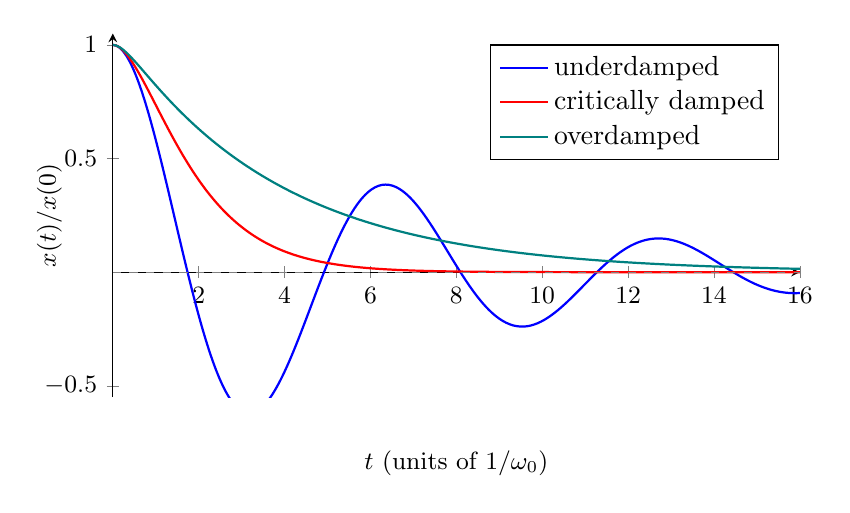
\begin{tikzpicture}
\begin{axis}[
    width=0.85\textwidth, height=6.2cm,
    xlabel={$t$ (units of $1/\omega_0$)}, ylabel={$x(t)/x(0)$},
    domain=0:16, samples=200,
    xmin=0, xmax=16, ymin=-0.55, ymax=1.05,
    axis lines=middle,
    every axis x label/.style={at={(axis description cs:0.5,-0.12)},anchor=north},
    every axis y label/.style={at={(axis description cs:-0.06,0.5)},rotate=90,anchor=south},
    legend pos=north east, legend cell align=left,
    tick label style={font=\small},
    label style={font=\small},
]
    % underdamped: gamma=0.15, omega=0.98869
    \addplot[thick, blue, smooth] {exp(-0.15*x)*(cos(deg(0.98869*x)) + (0.15/0.98869)*sin(deg(0.98869*x)))};
    \addlegendentry{underdamped}
    % critically damped: (1+t)e^{-t}
    \addplot[thick, red, smooth] {(1+x)*exp(-x)};
    \addlegendentry{critically damped}
    % overdamped: roots -0.2679, -3.7320
    \addplot[thick, teal, smooth] {(3.7320*exp(-0.2679*x) - 0.2679*exp(-3.7320*x))/3.4641};
    \addlegendentry{overdamped}
    \draw[gray, dashed] (axis cs:0,0) -- (axis cs:16,0);
\end{axis}
\end{tikzpicture}
\caption{Displacement of a damped oscillator released from rest at $x(0)$, for the three regimes (all with the same $\omega_0$). The underdamped case ($\Gamma/2 < \omega_0$) oscillates within a decaying envelope; the overdamped case ($\Gamma/2 > \omega_0$) returns monotonically but slowly; the critically damped case ($\Gamma/2 = \omega_0$) is the fastest non-oscillatory return.}
\label{fig:damped-decay}
\end{figure}

\begin{example}[Measuring $\Gamma$ from an underdamped decay envelope]
An underdamped mass on a spring is released and its amplitude is observed to drop to $1/e$ of its initial value after $N$ complete oscillations. What is the quality factor $Q = \omega_0/\Gamma$?

The envelope decays as $e^{-\Gamma t/2}$, and $N$ oscillations take time $t_N = 2\pi N/\omega \approx 2\pi N/\omega_0$ (valid when $Q \gg 1$, so $\omega \approx \omega_0$). Setting the envelope equal to $1/e$:
\begin{equation}
    \tfrac{\Gamma}{2}\cdot\frac{2\pi N}{\omega_0} = 1
    \quad\Longrightarrow\quad
    Q = \frac{\omega_0}{\Gamma} = \pi N.
\end{equation}
Counting rings against a stopwatch thus directly measures $Q$: a system that rings for ten full cycles before its amplitude falls to $1/e$ has $Q \approx 31$.
\end{example}

% ============================================================
\section{Forced Oscillations}
\label{sec:forced}
% ============================================================

So far the motion has been left to run down on its own. We now switch on the external drive $F(t)$ of Figure~\ref{fig:driven-schematic} and ask how the oscillator responds when energy is continually pumped in. The equation of motion becomes inhomogeneous:
\begin{equation}
    \ddot{x}(t) + \Gamma\,\dot{x}(t) + \omega_0^2\,x(t) = \frac{F(t)}{m}. \tag{$\ast$}
\end{equation}
We specialise to sinusoidal driving,
\begin{equation}
    F(t) = F_0\cos(\omega_d t),
\end{equation}
where $\omega_d$ is the driving angular frequency. To exploit linearity, complexify the drive as $F(t) = \operatorname{Re}\bigl\{F_0\,e^{-i\omega_d t}\bigr\}$ and seek a steady-state solution of the same form:
\begin{equation}
    z(t) = A\,e^{-i\omega_d t}.
\end{equation}
Notice: the steady-state response oscillates at the \emph{driving} frequency $\omega_d$, not at $\omega_0$ or $\omega$. The driving force entirely determines the steady-state behaviour.

Plugging into ($\ast$) and cancelling the common factor $e^{-i\omega_d t}$:
\begin{equation}
    (-\omega_d^2 - i\Gamma\omega_d + \omega_0^2)\,A = \frac{F_0}{m}
    \quad\Longrightarrow\quad
    A = \frac{F_0/m}{\omega_0^2 - i\Gamma\omega_d - \omega_d^2}.
\end{equation}
Rationalising by multiplying numerator and denominator by the complex conjugate of the denominator:
\begin{equation}
    A = \frac{F_0/m}{(\omega_0^2 - \omega_d^2)^2 + (\Gamma\omega_d)^2}\bigl[(\omega_0^2 - \omega_d^2) + i\,\Gamma\omega_d\bigr].
\end{equation}
Writing $A = A_e + iA_a$:
\begin{formula}
\begin{align}
    A_e &= \frac{F_0}{m}\,\frac{\omega_0^2 - \omega_d^2}{(\omega_0^2 - \omega_d^2)^2 + (\Gamma\omega_d)^2} \qquad\text{(elastic amplitude),}\\
    A_a &= \frac{F_0}{m}\,\frac{\Gamma\omega_d}{(\omega_0^2 - \omega_d^2)^2 + (\Gamma\omega_d)^2} \qquad\text{(absorptive amplitude).}
\end{align}
\end{formula}

The complex steady-state solution is
\begin{equation}
    z(t) = A\,e^{-i\omega_d t} = (A_e + iA_a)\,e^{-i\omega_d t},
\end{equation}
and its real part gives the physical displacement
\begin{formula}
\begin{equation}
    x_p(t) = \operatorname{Re}\{z(t)\} = A_e\cos(\omega_d t) + A_a\sin(\omega_d t).
\end{equation}
\end{formula}

\subsection{Amplitude and Phase Behaviour}

Writing $x_p(t) = R\cos(\omega_d t - \delta)$ with $R = \sqrt{A_e^2 + A_a^2}$ and $\tan\delta = A_a/A_e$:
\begin{formula}
\begin{align}
    R(\omega_d) &= \frac{F_0/m}{\sqrt{(\omega_0^2 - \omega_d^2)^2 + (\Gamma\omega_d)^2}}, \\
    \delta(\omega_d) &= \arctan\!\left(\frac{\Gamma\omega_d}{\omega_0^2 - \omega_d^2}\right).
\end{align}
\end{formula}
The limits are transparent. For $\omega_d \to 0$, $R \to F_0/(m\omega_0^2)$, the static response of the spring to a steady force; for $\omega_d \to \infty$, $R \to 0$, since the mass cannot keep up with an infinitely rapid drive. Between these extremes the amplitude rises to a pronounced peak near $\omega_d = \omega_0$, the sharper the weaker the damping; Figure~\ref{fig:resonance-amp} shows the curve for several quality factors $Q = \omega_0/\Gamma$.

The phase lag $\delta$ tells a complementary story, sweeping from $0$ at low $\omega_d$, through $\pi/2$ exactly at $\omega_d = \omega_0$, up to $\pi$ at high $\omega_d$ (Figure~\ref{fig:phase-lag}). It is cleanest to read $\delta = \arg(A_e + iA_a)$ as the argument of the response vector $(A_e, A_a)$. The absorptive part $A_a \propto \Gamma\omega_d$ is positive for all $\omega_d > 0$, so the vector always lies in the upper half plane. The elastic part $A_e \propto \omega_0^2 - \omega_d^2$ changes sign at resonance: below resonance $A_e > 0$ and the vector sits in the first quadrant ($0 < \delta < \pi/2$); above resonance $A_e < 0$ and it swings into the second quadrant ($\pi/2 < \delta < \pi$). As $\omega_d \to \infty$ the vector approaches the negative real axis, so $\delta \to \pi$. The lighter the damping, the more abruptly this swing occurs.

\begin{figure}[ht]
\centering
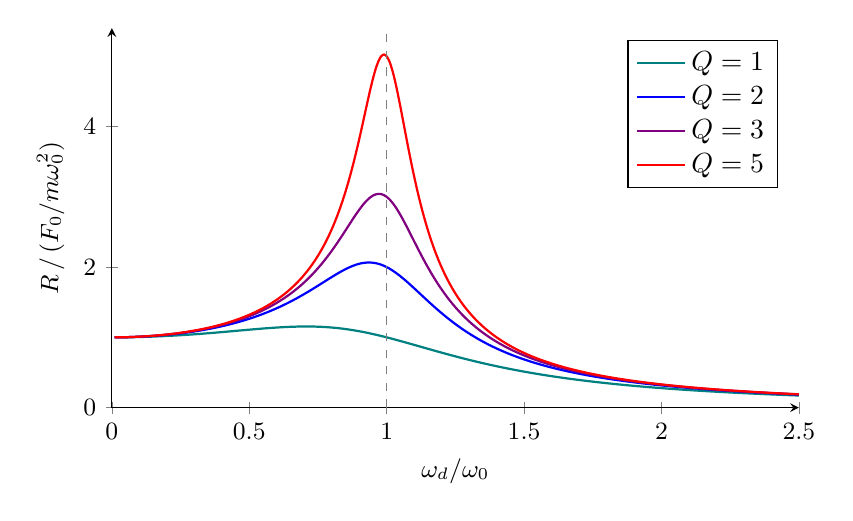
\begin{tikzpicture}
\begin{axis}[
    width=0.85\textwidth, height=6.4cm,
    xlabel={$\omega_d/\omega_0$}, ylabel={$R \,/\, (F_0/m\omega_0^2)$},
    domain=0.01:2.5, samples=250,
    xmin=0, xmax=2.5, ymin=0, ymax=5.4,
    axis lines=left,
    legend pos=north east, legend cell align=left,
    tick label style={font=\small},
    label style={font=\small},
]
    % R = 1/sqrt((1-u^2)^2 + (u/Q)^2), amplitude normalized to static value (=1 at u=0)
    \addplot[thick, teal, smooth]   {1/sqrt((1-x^2)^2 + (x/1)^2)};
    \addlegendentry{$Q=1$}
    \addplot[thick, blue, smooth]   {1/sqrt((1-x^2)^2 + (x/2)^2)};
    \addlegendentry{$Q=2$}
    \addplot[thick, violet, smooth] {1/sqrt((1-x^2)^2 + (x/3)^2)};
    \addlegendentry{$Q=3$}
    \addplot[thick, red, smooth]    {1/sqrt((1-x^2)^2 + (x/5)^2)};
    \addlegendentry{$Q=5$}
    \draw[gray, dashed] (axis cs:1,0) -- (axis cs:1,5.4);
\end{axis}
\end{tikzpicture}
\caption{Steady-state amplitude $R$ versus driving frequency $\omega_d$, normalized to the static response $F_0/(m\omega_0^2)$, for several quality factors $Q = \omega_0/\Gamma$. Higher $Q$ (weaker damping) gives a taller, narrower resonance peak near $\omega_d = \omega_0$ (dashed line).}
\label{fig:resonance-amp}
\end{figure}

\begin{figure}[ht]
\centering
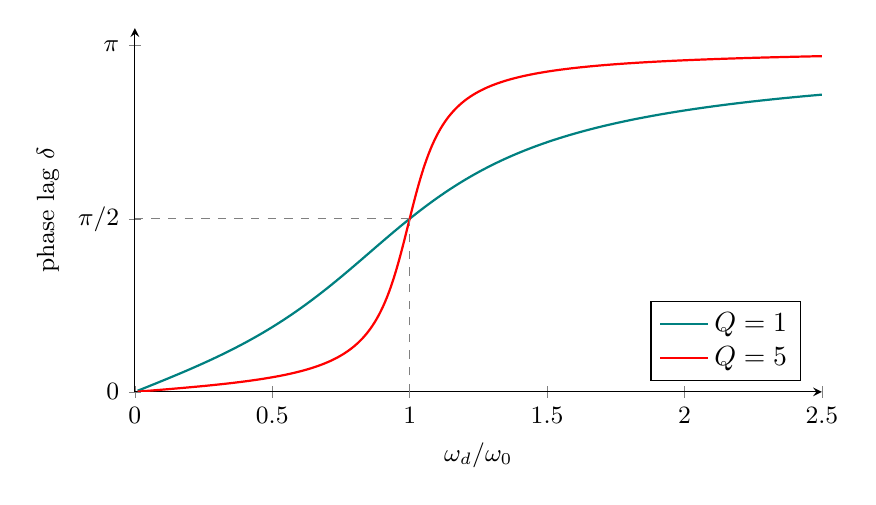
\begin{tikzpicture}
\begin{axis}[
    width=0.85\textwidth, height=6.2cm,
    xlabel={$\omega_d/\omega_0$}, ylabel={phase lag $\delta$},
    domain=0.01:2.5, samples=250,
    xmin=0, xmax=2.5, ymin=0, ymax=3.3,
    axis lines=left,
    ytick={0, 1.5707963, 3.1415926},
    yticklabels={$0$, $\pi/2$, $\pi$},
    legend pos=south east, legend cell align=left,
    tick label style={font=\small},
    label style={font=\small},
]
    % delta = atan2(Gamma*wd, w0^2 - wd^2) in radians; Gamma = 1/Q
    \addplot[thick, teal, smooth] {atan2(x/1, 1-x^2)*pi/180};
    \addlegendentry{$Q=1$}
    \addplot[thick, red, smooth]  {atan2(x/5, 1-x^2)*pi/180};
    \addlegendentry{$Q=5$}
    \draw[gray, dashed] (axis cs:1,0) -- (axis cs:1,1.5707963);
    \draw[gray, dashed] (axis cs:0,1.5707963) -- (axis cs:1,1.5707963);
\end{axis}
\end{tikzpicture}
\caption{Phase lag $\delta$ of the steady-state response behind the drive, as a function of driving frequency. The response is in phase at low $\omega_d$, lags by exactly $\pi/2$ at resonance $\omega_d = \omega_0$ (dashed lines), and approaches $\pi$ (fully out of phase) at high $\omega_d$. Lighter damping (higher $Q$) makes the transition through $\pi/2$ steeper.}
\label{fig:phase-lag}
\end{figure}

% ============================================================
\section{Resonance}
% ============================================================

The amplitude peak of Figure~\ref{fig:resonance-amp} is the visible face of resonance, but its physical origin is best understood through energy: resonance is the frequency at which the drive delivers power to the oscillator most efficiently. We therefore compute the work done by the driving force, identify the frequency that maximizes it, and read off the width of the resulting peak.

\subsection{Work Done by the Driving Force}

The instantaneous power delivered to the oscillator by the driving force is
\begin{equation}
    P(t) = F(t)\,\dot{x}_p(t)
    = F_0\cos(\omega_d t)\,\bigl[-A_e\omega_d\sin(\omega_d t) + A_a\omega_d\cos(\omega_d t)\bigr].
\end{equation}
Distributing:
\begin{equation}
    P(t) = -F_0\omega_d A_e\,\tfrac{1}{2}\sin(2\omega_d t) + F_0\omega_d A_a\cos^2(\omega_d t).
\end{equation}
The first term has period $\pi/\omega_d$ and averages to zero over a full drive period (this is why $A_e$ is called the \emph{elastic} amplitude: it stores and returns energy). The second term is always positive; averaging $\cos^2$ to $1/2$ gives the mean absorbed power
\begin{equation}
    P_\text{avg} = \tfrac{1}{2}F_0\omega_d A_a
    = \tfrac{1}{2}F_0\omega_d \cdot \frac{F_0}{m}\,\frac{\Gamma\omega_d}{(\omega_0^2 - \omega_d^2)^2 + (\Gamma\omega_d)^2}.
\end{equation}
\begin{formula}
\begin{equation}
    P_\text{avg}(\omega_d) = \frac{F_0^2\,\omega_d^2\,\Gamma}{2m\bigl[(\omega_0^2 - \omega_d^2)^2 + (\Gamma\omega_d)^2\bigr]}.
\end{equation}
\end{formula}
This is the \emph{resonance curve}: absorbed power as a function of driving frequency.

\subsection{Resonance Width and Lifetime}

The maximum average power is delivered at $\omega_d = \omega_0$:
\begin{equation}
    P_\text{max} = \frac{F_0^2}{2m\Gamma}.
\end{equation}
The \emph{half-power frequencies} $\omega_{1/2}$ satisfy $P_\text{avg}(\omega_{1/2}) = P_\text{max}/2$. Setting this ratio and simplifying:
\begin{align}
    (\omega_0^2 - \omega_d^2)^2 + (\Gamma\omega_d)^2 &= 2\omega_d^2\Gamma^2 \\
    (\omega_0^2 - \omega_d^2)^2 &= \omega_d^2\Gamma^2 \\
    \omega_0^2 - \omega_d^2 &= \pm\omega_d\Gamma \\
    \omega_0^2 + \tfrac{\Gamma^2}{4} &= \bigl(\omega_d \pm \tfrac{\Gamma}{2}\bigr)^2.
\end{align}
Solving for $\omega_d$ at the half-power points:
\begin{formula}
\begin{equation}
    \omega_{1/2} = \sqrt{\omega_0^2 + \tfrac{\Gamma^2}{4}}\,\pm\,\tfrac{\Gamma}{2}.
\end{equation}
\end{formula}
The full width at half maximum (FWHM) of the resonance curve is therefore exactly $\Gamma$. This is a remarkable economy: the damping rate simultaneously controls (i) the transient decay lifetime $\tau = 2/\Gamma$ and (ii) the resonance width. A weakly damped oscillator rings for a long time \emph{and} responds only to a narrow band of frequencies --- the two statements are one and the same, as the progression toward taller, narrower peaks in Figure~\ref{fig:resonance-amp} makes visible.

\subsection{Phase Lag}

Recall the form of the steady-state displacement,
\begin{equation}
    x_p(t) = R\cos(\omega_d t - \delta), \qquad R = \sqrt{A_e^2 + A_a^2},\quad \delta = \arg(A_e + iA_a).
\end{equation}
Factoring $\omega_d$ out of the argument,
\begin{equation}
    x_p(t) = R\cos\!\left(\omega_d\bigl(t - \tfrac{\delta}{\omega_d}\bigr)\right),
\end{equation}
so the driven response lags the drive by a \emph{time lag} $\delta/\omega_d$. Weaker damping produces sharper resonance peaks (least damping $\Rightarrow$ tallest, narrowest curve) and, correspondingly, a more abrupt swing of the phase $\delta$ through $\pi/2$ near $\omega_0$, as the $Q=5$ curve of Figure~\ref{fig:phase-lag} shows.

\subsection{Quality of a Damped Oscillator}

\begin{definition}[Quality factor]
The dimensionless quality factor of a damped oscillator is
\begin{equation}
    Q \defeq \frac{\omega_0}{\Gamma}.
\end{equation}
Physically, $Q$ is proportional to the reciprocal of the fractional energy lost per cycle:
\begin{equation}
    Q \propto \frac{1}{\text{(system energy loss per cycle)}/\text{(energy stored)}}.
\end{equation}
\end{definition}

Ringing of a lightly damped oscillator therefore extends over $\sim Q$ cycles before decaying appreciably.

\begin{example}[Wine glass vs. table]
A wine glass has a high quality factor---struck, it rings for many cycles. A wooden table has a very low quality factor---struck, it produces a dull thud that dies within a fraction of a period.
\end{example}

% ============================================================
\section{Energy Dissipation and Steady State}
% ============================================================

We can verify the resonance formula from an energy-balance argument. The total mechanical energy is
\begin{equation}
    E = K + V = \tfrac{1}{2}m\dot{x}^2 + \tfrac{1}{2}kx^2,
\end{equation}
so
\begin{equation}
    \dot{E} = m\dot{x}\ddot{x} + kx\dot{x} = \dot{x}\bigl(m\ddot{x} + kx\bigr).
\end{equation}
Substituting the driven equation of motion $m\ddot{x} + kx = -m\Gamma\dot{x} + F_0\cos(\omega_d t)$ gives
\begin{equation}
    \dot{E} = -m\Gamma\,\dot{x}^2 + F_0\cos(\omega_d t)\,\dot{x}(t).
\end{equation}
In steady state, $\dot{E}$ averages to zero over a cycle: the power delivered by the drive is exactly balanced by the power dissipated by friction, $\langle F_0\cos(\omega_d t)\,\dot{x}\rangle = m\Gamma\langle \dot{x}^2\rangle$. The full solution decomposes as
\begin{equation}
    x(t) = x_\text{transient}(t) + x_\text{steady-state}(t),
\end{equation}
where $x_\text{transient}$ is the homogeneous solution (decays on time $2/\Gamma$) and $x_\text{steady-state}$ is the driven particular solution.

\subsection{Low- and High-Frequency Regimes}

The three terms $m\ddot{x}$, $m\Gamma\dot{x}$, and $kx$ compete inside the equation of motion, and it is instructive to ask which of them the drive must balance at a given $\omega_d$. Substituting the steady-state ansatz $x \sim \cos(\omega_d t)$ gives $\dot{x} \sim -\omega_d\sin(\omega_d t)$ and $\ddot{x} \sim -\omega_d^2\cos(\omega_d t)$, so the three terms scale as $m\omega_d^2$, $m\Gamma\omega_d$, and $k$ respectively.

At low driving frequency, $\omega_d \ll \omega_0$, the constant $k$ dwarfs both $m\omega_d^2$ and $m\Gamma\omega_d$, so the drive is balanced almost entirely by the spring: $kx \approx F_0\cos(\omega_d t)$. The mass follows the drive quasi-statically, in phase with it, and the phase lag $\delta$ is nearly zero. In the opposite limit, $\omega_d \gg \omega_0$, inertia dominates: $m\ddot{x} \approx F_0\cos(\omega_d t)$, so $x \sim -\cos(\omega_d t)/\omega_d^2$. The mass is too heavy to keep up, and it moves oppositely to the drive at any instant, so $\delta \approx \pi$. The two limits are separated by a crossover exactly at $m\omega_d^2 \sim k$, i.e.\ $\omega_d = \omega_0$; there the inertial and restoring terms cancel identically, and the drive is balanced only by damping,
\begin{equation}
    m\Gamma\dot{x} = F_0\cos(\omega_d t) \;\Longrightarrow\; x \sim \sin(\omega_d t) = \cos(\omega_d t - \pi/2).
\end{equation}
This is why the phase lag passes through exactly $\pi/2$ at resonance: it is the frequency at which the mass has stopped following the drive but has not yet begun to oppose it, and the only force left to push against is friction.

\begin{example}[Driven RLC circuit at half-power]
A series RLC circuit with $L=10\text{ mH}$, $C=1\,\mu\text{F}$, $R=20\,\Omega$ is driven by an EMF source $\mathcal{E}(t) = \mathcal{E}_0\cos(\omega_d t)$. Find the resonance frequency, quality factor, and FWHM of the absorbed-power curve.

Under the analogy $L\leftrightarrow m$, $R\leftrightarrow m\Gamma$, $1/C\leftrightarrow k$, the natural frequency and damping rate read
\begin{equation}
    \omega_0 = \frac{1}{\sqrt{LC}} = 10^4\text{ rad/s},\qquad \Gamma = \frac{R}{L} = 2\times 10^3\text{ s}^{-1}.
\end{equation}
The quality factor is $Q = \omega_0/\Gamma = 5$, and the FWHM of the resonance curve equals $\Gamma = 2\times 10^3\text{ rad/s}$. The circuit therefore rings for roughly $Q/\pi\approx 1.6$ cycles after the drive is switched off, and its bandwidth around resonance is narrow but not sharp.
\end{example}

\subsection{Steady-State Energetics at Resonance}

For $x_\text{ss}(t) = A'\cos(\omega_d t + \varphi')$, the kinetic and potential energies are
\begin{align}
    K &= \tfrac{1}{2}mA'^2\omega_d^2\sin^2(\omega_d t + \varphi'), \\
    V &= \tfrac{1}{2}kA'^2\cos^2(\omega_d t + \varphi').
\end{align}
At $\omega_d = \omega_0$, the two amplitude coefficients $\tfrac{1}{2}mA'^2\omega_d^2$ and $\tfrac{1}{2}kA'^2$ coincide (since $k = m\omega_0^2$), so the total mechanical energy is constant in time: $K + V = \tfrac{1}{2}kA'^2$. All work done by the drive is dissipated by damping; none accumulates as growth of the oscillation amplitude.

\begin{example}[Energy loss per cycle and the meaning of $Q$]
A lightly damped driven oscillator sits in steady state at resonance with amplitude $A'$. Compute the energy stored, the energy dissipated per cycle, and verify the interpretation of $Q$.

The stored energy is $E = \tfrac{1}{2}kA'^2 = \tfrac{1}{2}m\omega_0^2 A'^2$. The instantaneous dissipation rate is $m\Gamma \dot{x}^2$; averaged over a cycle at $\omega_d = \omega_0$,
\begin{equation}
    \langle P_\text{diss}\rangle = m\Gamma\,\langle \dot{x}^2\rangle = m\Gamma\cdot\tfrac{1}{2}\omega_0^2 A'^2 = \Gamma E.
\end{equation}
The energy lost per period $T = 2\pi/\omega_0$ is therefore $\Delta E = \Gamma E\cdot 2\pi/\omega_0$, so
\begin{equation}
    \frac{\Delta E}{E} = \frac{2\pi\Gamma}{\omega_0} = \frac{2\pi}{Q},
\end{equation}
confirming that $Q$ is $2\pi$ times the ratio of stored energy to energy lost per cycle. A wine glass with $Q\sim 10^3$ loses less than one part in a hundred of its ring energy per period.
\end{example}

% ============================================================
\section{Circuit Analogues}
% ============================================================

The RLC circuit is the electrical analogue of the damped, driven oscillator. Kirchhoff's voltage law around a loop, with a chosen circulation direction, sums signed potential drops to zero. Recall the constitutive relations for the three passive elements:
\begin{fact}[Circulation voltage rules]
For a resistor, inductor, and capacitor in a loop:
\begin{align}
    \Delta V_R(t) &= R\,I(t), \\
    \Delta V_L(t) &= L\,\dot{I}(t), \\
    \Delta V_C(t) &= \frac{Q(t)}{C}.
\end{align}
When traversing the element in the direction of assumed positive current, the potential ``drops'' across a resistor or inductor---subtract $\Delta V$ from the circulating potential. For a capacitor, traversing from the ``$-$'' plate to the ``$+$'' plate \emph{adds} $Q/C$; going from ``$+$'' to ``$-$'' \emph{subtracts} it.
\end{fact}
The sign of $I = \pm\,\dv{Q}{t}$ depends on the orientation of $I$ relative to the capacitor plates: if positive current flows \emph{into} the positive plate, $I = +\dv{Q}{t}$; if positive current flows \emph{out} of the positive plate, $I = -\dv{Q}{t}$. With these rules the RLC loop equation takes the form of the forced damped oscillator with $L \leftrightarrow m$, $R \leftrightarrow m\Gamma$, $1/C \leftrightarrow k$, and drive supplied by an EMF source.
